
\chapter{Validation}
\label{chp:NumMethodComp}

\section{Analytic Validation}

\subsection{Soliton}
%C1, H1 and L1

%$a0 = 1$
%$a1 = 0.7$

\begin{figure}
	\centering
	\begin{subfigure}{0.5\textwidth}
		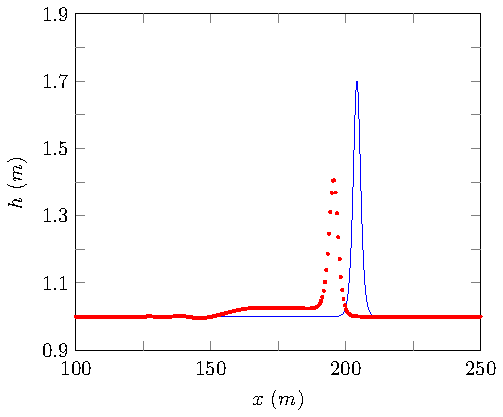
\includegraphics[width=\textwidth]{./chp5/figures/Analytic/Soliton/Example/FDVM1.pdf}
		\subcaption{$\text{FDVM}_1$}
	\end{subfigure}%
	\begin{subfigure}{0.5\textwidth}
		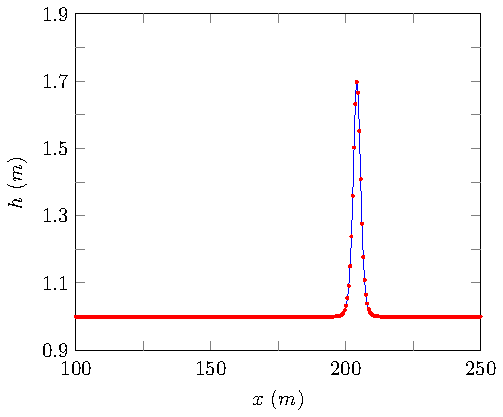
\includegraphics[width=\textwidth]{./chp5/figures/Analytic/Soliton/Example/FDVM2.pdf}
		\subcaption{$\text{FDVM}_2$}
	\end{subfigure}
	\begin{subfigure}{0.5\textwidth}
		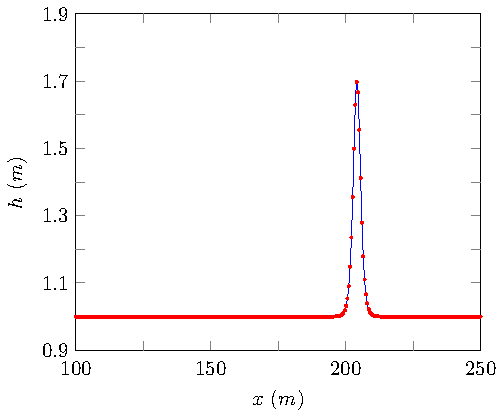
\includegraphics[width=\textwidth]{./chp5/figures/Analytic/Soliton/Example/FEVM2.pdf}
		\subcaption{$\text{FEVM}_2$}
	\end{subfigure}%
	\begin{subfigure}{0.5\textwidth}
		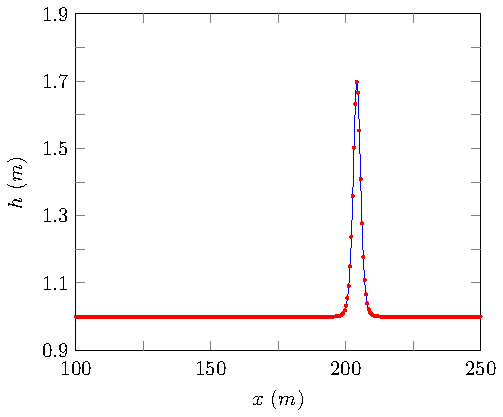
\includegraphics[width=\textwidth]{./chp5/figures/Analytic/Soliton/Example/FDVM3.pdf}
		\subcaption{$\text{FDVM}_3$}
	\end{subfigure}
	\begin{subfigure}{0.5\textwidth}
		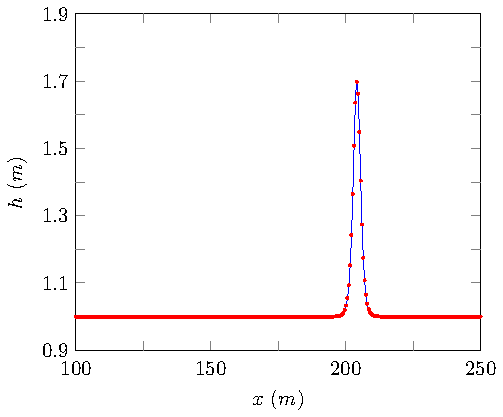
\includegraphics[width=\textwidth]{./chp5/figures/Analytic/Soliton/Example/D.pdf}
		\subcaption{$\mathcal{D}$}
	\end{subfigure}%
	\begin{subfigure}{0.5\textwidth}
		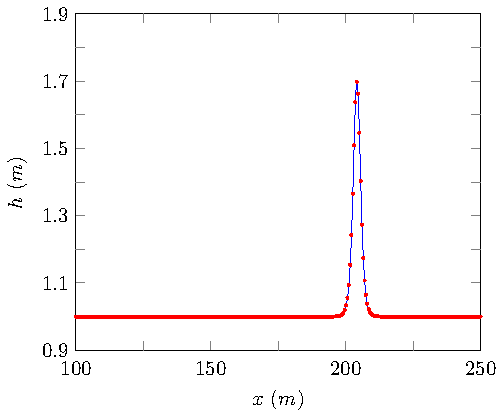
\includegraphics[width=\textwidth]{./chp5/figures/Analytic/Soliton/Example/W.pdf}
		\subcaption{$\mathcal{W}$}
	\end{subfigure}
	\caption{Example soliton with $\Delta x = \frac{100}{2^{11}}$. Red dots numerical, solid blue analytic.}
	\label{fig:SolitonExAll}
\end{figure}

\begin{figure}
	\centering
	\begin{subfigure}{0.5\textwidth}
		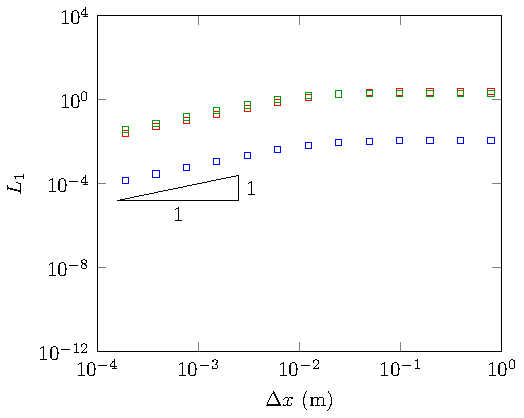
\includegraphics[width=\textwidth]{./chp5/figures/Analytic/Soliton/L1/FDVM1.pdf}
		\subcaption{$\text{FDVM}_1$}
	\end{subfigure}%
	\begin{subfigure}{0.5\textwidth}
		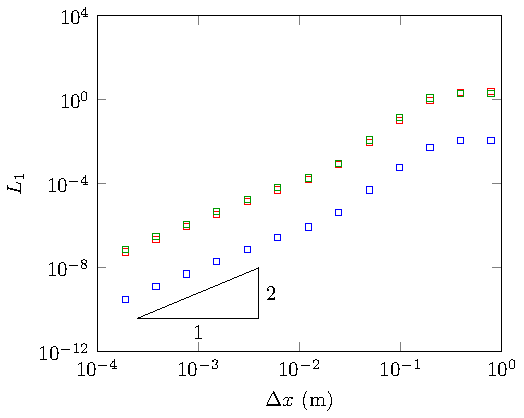
\includegraphics[width=\textwidth]{./chp5/figures/Analytic/Soliton/L1/FDVM2.pdf}
		\subcaption{$\text{FDVM}_2$}
	\end{subfigure}
	\begin{subfigure}{0.5\textwidth}
		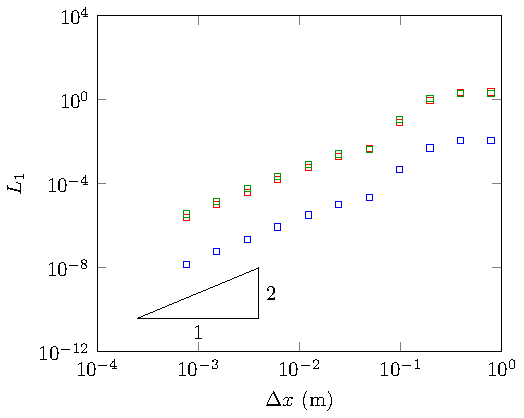
\includegraphics[width=\textwidth]{./chp5/figures/Analytic/Soliton/L1/FEVM2.pdf}
		\subcaption{$\text{FEVM}_2$}
	\end{subfigure}%
	\begin{subfigure}{0.5\textwidth}
		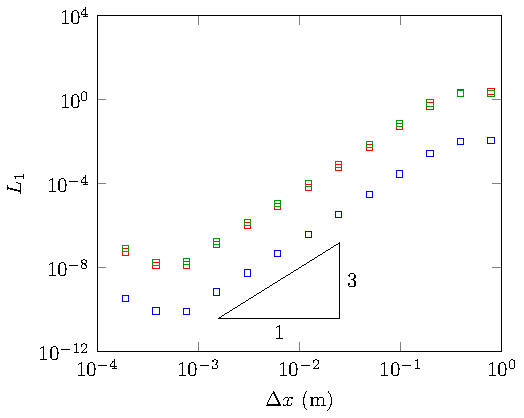
\includegraphics[width=\textwidth]{./chp5/figures/Analytic/Soliton/L1/FDVM3.pdf}
		\subcaption{$\text{FDVM}_3$}
	\end{subfigure}
	\begin{subfigure}{0.5\textwidth}
		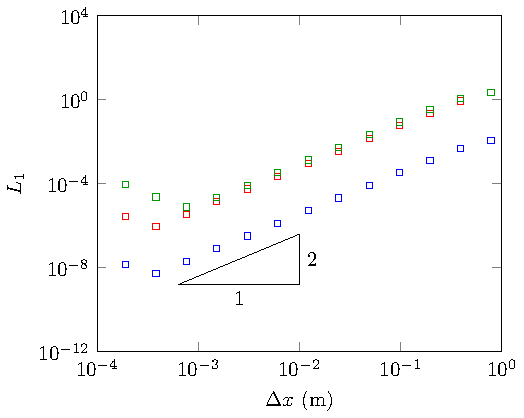
\includegraphics[width=\textwidth]{./chp5/figures/Analytic/Soliton/L1/D.pdf}
		\subcaption{$\mathcal{D}$}
	\end{subfigure}%
	\begin{subfigure}{0.5\textwidth}
		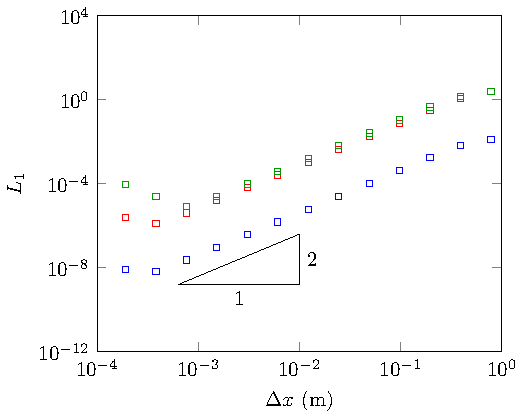
\includegraphics[width=\textwidth]{./chp5/figures/Analytic/Soliton/L1/W.pdf}
		\subcaption{$\mathcal{W}$}
	\end{subfigure}
	\caption{$L1$. Blue h, red u, green G.}
	\label{fig:SolitonL1All}
\end{figure}

\begin{figure}
	\centering
	\begin{subfigure}{0.5\textwidth}
		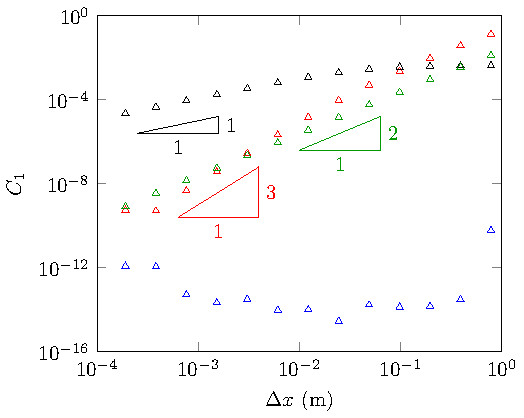
\includegraphics[width=\textwidth]{./chp5/figures/Analytic/Soliton/C1/FDVM1.pdf}
		\subcaption{$\text{FDVM}_1$}
	\end{subfigure}%
	\begin{subfigure}{0.5\textwidth}
		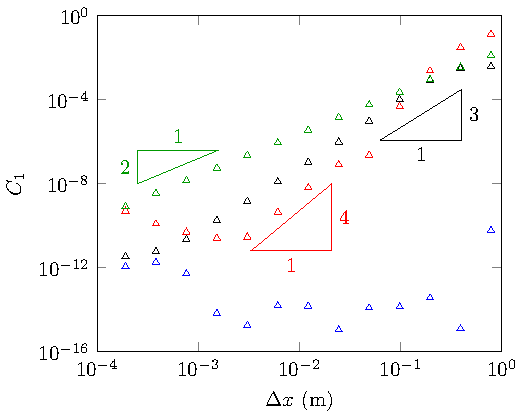
\includegraphics[width=\textwidth]{./chp5/figures/Analytic/Soliton/C1/FDVM2.pdf}
		\subcaption{$\text{FDVM}_2$}
	\end{subfigure}
	\begin{subfigure}{0.5\textwidth}
		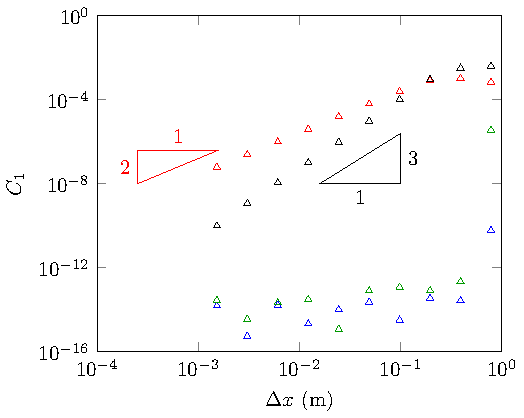
\includegraphics[width=\textwidth]{./chp5/figures/Analytic/Soliton/C1/FEVM2.pdf}
		\subcaption{$\text{FEVM}_2$}
	\end{subfigure}%
	\begin{subfigure}{0.5\textwidth}
		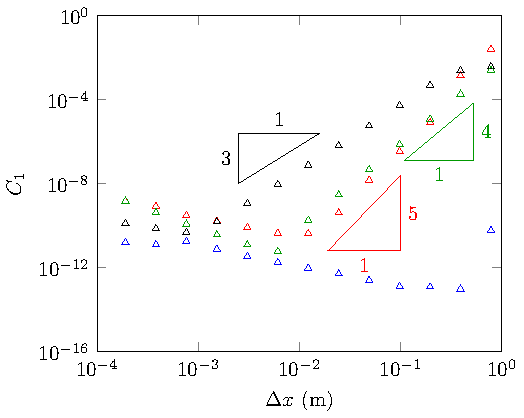
\includegraphics[width=\textwidth]{./chp5/figures/Analytic/Soliton/C1/FDVM3.pdf}
		\subcaption{$\text{FDVM}_3$}
	\end{subfigure}
	\begin{subfigure}{0.5\textwidth}
		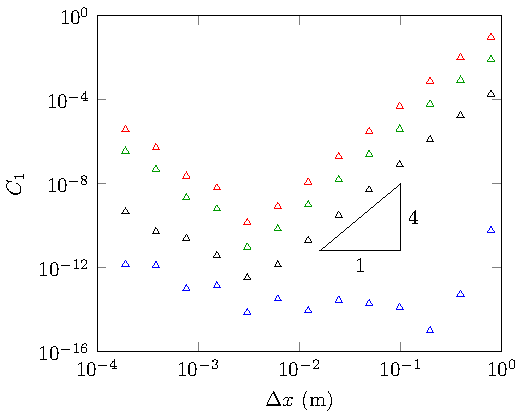
\includegraphics[width=\textwidth]{./chp5/figures/Analytic/Soliton/C1/D.pdf}
		\subcaption{$\mathcal{D}$}
	\end{subfigure}%
	\begin{subfigure}{0.5\textwidth}
		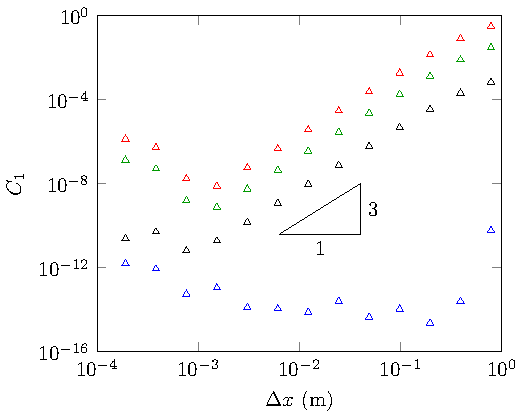
\includegraphics[width=\textwidth]{./chp5/figures/Analytic/Soliton/C1/W.pdf}
		\subcaption{$\mathcal{W}$}
	\end{subfigure}
	\caption{$C1$. Blue h, red u, black $\mathcal{H}$, green G.}
	\label{fig:SolitonC1All}
\end{figure}

\subsection{Lake at Rest}
%C1, H1 and L1

\section{Forced Solutions}
%only L1





\subsection{Travelling Gaussian}
\begin{equation}
h(x,t) = a_0 + a_1\exp\left(-\dfrac{ \left(\left(x - a_2t\right) - a_3 \right)^2}{2a_4}\right)
\end{equation}
\begin{equation}
u(x,t) = a_5\exp\left(-\dfrac{ \left(\left(x - a_2t\right) - a_3 \right)^2}{2a_4}\right)
\end{equation}
\begin{equation}
b(x) = a_6\sin\left(a_7 x\right)
\end{equation}

%With $a_0 = 1$ or $a_0 = 0$.
%$a_1 = 0.5$
%$a_2 = 1$
%$a3 = -20$
%$a4 = 1$
%$a5 = a1$
%$a6 = 1$
%$a7 = 0.1$
%$x \in \left[- \frac{\pi}{a_9} , 0\right]$
%$Cr = 0.5$
%$\Delta t = \frac{Cr}{a_5 + \sqrt{g \left(a_0 + a_1\right)}} \Delta x$
%$et = 1$

% Give the source terms for these functions

%Equation for G

% Give the source terms for these functions

%ht

%Gt

%fluxh

%fluxG

%Source G

\begin{figure}
	\centering
	\begin{subfigure}{0.5\textwidth}
		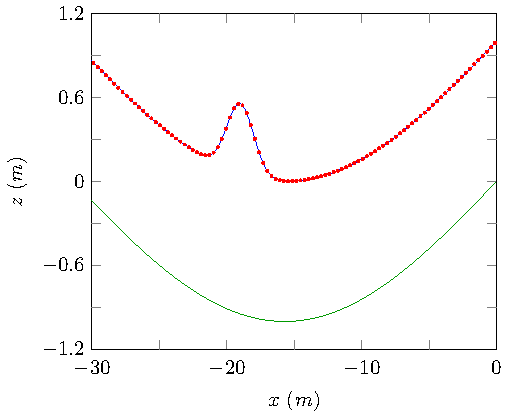
\includegraphics[width=\textwidth]{./chp5/figures/Forced/Wet/exFDVM2.pdf}
		\subcaption{$\text{FDVM}_2$}
	\end{subfigure}%
	\begin{subfigure}{0.5\textwidth}
		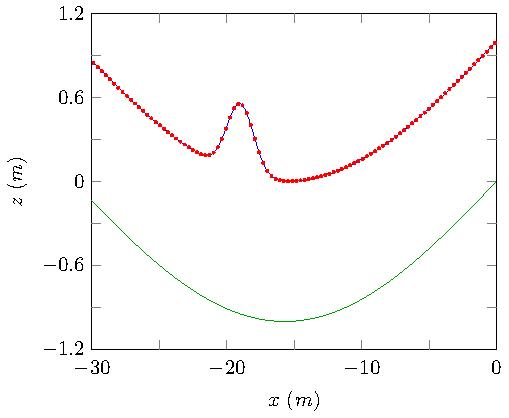
\includegraphics[width=\textwidth]{./chp5/figures/Forced/Wet/exFEVM2.pdf}
		\subcaption{$\text{FEVM}_2$}
	\end{subfigure}
	\caption{Example with $\Delta x = \frac{100}{2^{11}}$ $a_0 = 1$. Red dots numerical, solid blue analytic..}
	\label{fig:TravGaussWetexAll}
\end{figure}

\begin{figure}
	\centering
	\begin{subfigure}{0.5\textwidth}
		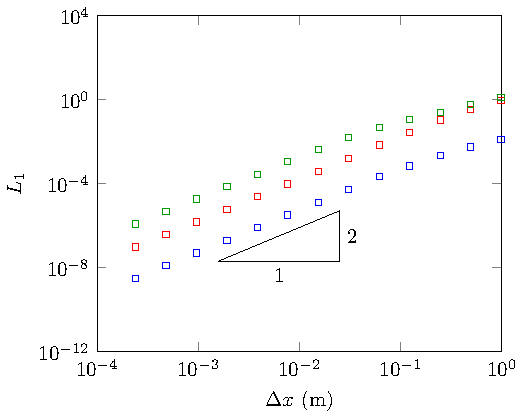
\includegraphics[width=\textwidth]{./chp5/figures/Forced/Wet/FDVM2.pdf}
		\subcaption{$\text{FDVM}_2$}
	\end{subfigure}%
	\begin{subfigure}{0.5\textwidth}
		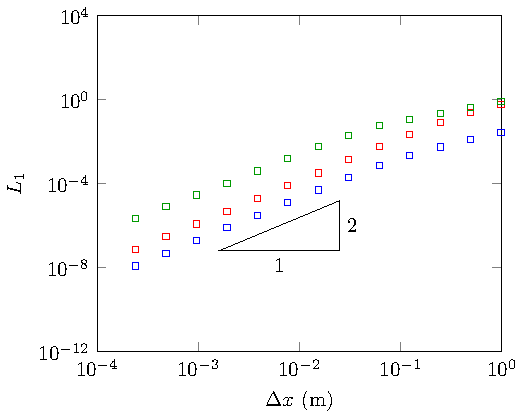
\includegraphics[width=\textwidth]{./chp5/figures/Forced/Wet/FEVM2.pdf}
		\subcaption{$\text{FEVM}_2$}
	\end{subfigure}
	\caption{$L1$ $a_0 = 1$ Blue h, red u, green G..}
	\label{fig:TravGaussWetL1All}
\end{figure}

\begin{figure}
	\centering
	\begin{subfigure}{0.5\textwidth}
		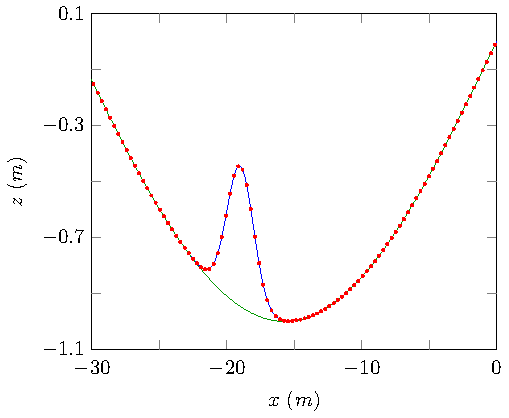
\includegraphics[width=\textwidth]{./chp5/figures/Forced/Dry/exFDVM2.pdf}
		\subcaption{$\text{FDVM}_2$}
	\end{subfigure}%
	\begin{subfigure}{0.5\textwidth}
		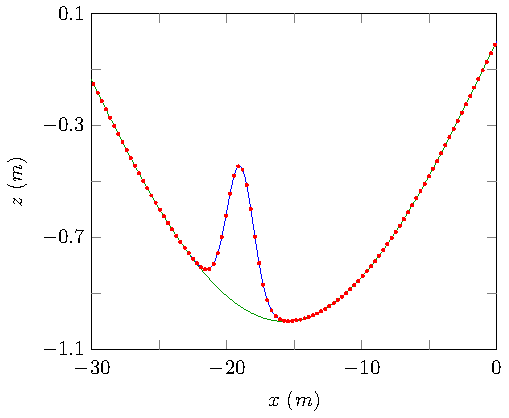
\includegraphics[width=\textwidth]{./chp5/figures/Forced/Dry/exFEVM2.pdf}
		\subcaption{$\text{FEVM}_2$}
	\end{subfigure}
	\caption{Example with $\Delta x = \frac{100}{2^{11}}$ $a_0 = 0$. Red dots numerical, solid blue analytic..}
	\label{fig:TravGaussDryexAll}
\end{figure}

\begin{figure}
	\centering
	\begin{subfigure}{0.5\textwidth}
		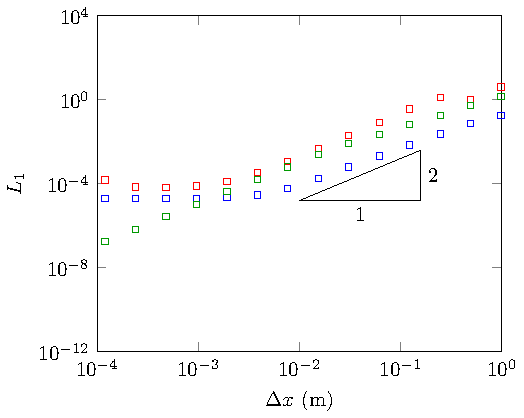
\includegraphics[width=\textwidth]{./chp5/figures/Forced/Dry/FDVM2.pdf}
		\subcaption{$\text{FDVM}_2$}
	\end{subfigure}%
	\begin{subfigure}{0.5\textwidth}
		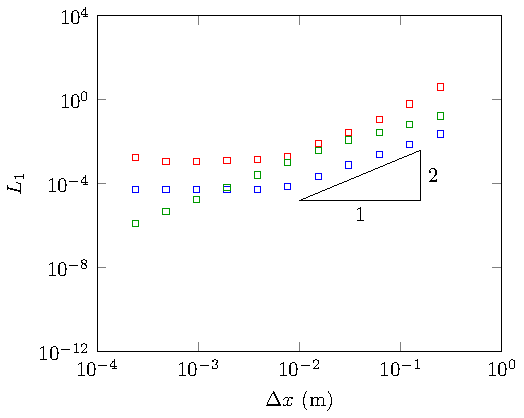
\includegraphics[width=\textwidth]{./chp5/figures/Forced/Dry/FEVM2.pdf}
		\subcaption{$\text{FEVM}_2$}
	\end{subfigure}
\caption{$L1$ $a_0 = 0$ Blue h, red u, green G..}
\label{fig:TravGaussDryL1All}
\end{figure}


\section{Experimental Validation}

\subsection{Beji}
%only pointwise comparison

\subsection{Synolakis}
%only pointwise comparison, and H1 and C1 as wave is well defined

\subsection{Roeber}
%only pointwise comparison
